% graph articulation point
% https://www.geeksforgeeks.org/articulation-points-or-cut-vertices-in-a-graph/
% https://www.hackerearth.com/practice/algorithms/graphs/articulation-points-and-bridges/tutorial/
% http://www.cs.kent.edu/~aleitert/iga/slides/04ArtPointsBridges.pdf
% https://iq.opengenus.org/find-articulation-points-or-cut-vertices-in-a-graph/
% https://cp-algorithms.com/graph/cutpoints.html
% https://www.codechef.com/problems/KINGCON
% https://www.hackerearth.com/practice/notes/nj/
% Introduction to Algorithms 3rd Edition - Page 621
% https://onlinejudge.org/index.php?option=com_onlinejudge&Itemid=8&category=670

% http://www.cs.kent.edu/~aleitert/iga/slides/04ArtPointsBridges.pdf
\section{Puntos de articulación}\label{articulation-points}
Un vértice \( v \) es un punto de articulación (o vértice de corte), si al eliminar el vértice \( v \) del grafo aumenta el número de componentes conectados. Es decir, genera algunos vértices inalcanzables para otros, se desconecta el grafo \cite{Jaimini2017}.

\begin{figure}[H]
	\centering
	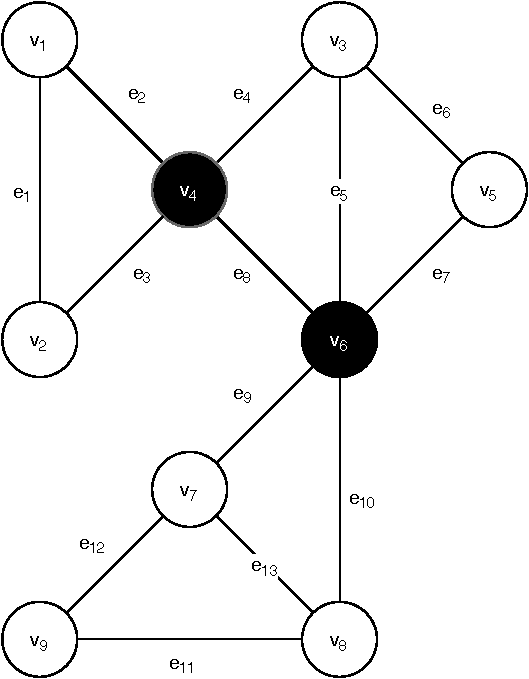
\includegraphics[width=0.4\linewidth]{document/ArticulationPoints/images/example-of-articulation-points}
	\caption{Ejemplo de grafo con dos puntos de articulación \( v_4 \) y \( v_6 \).}
	\label{fig:connected-disconnected-graph}
\end{figure}

% Encontrar los algoritmos que me permitan determinar en un grafo cuales son los nodos, en ultimas si los quito la cosa queda disconexa, una masa viscosa de puntos, otra masa viscosa de puntos, se tocan en un solo punto, el grafo es conexo, si yo quito ese nodo, entonces se partió en dos, esos puntos son claves en redes.

% https://www.geeksforgeeks.org/articulation-points-or-cut-vertices-in-a-graph/
% https://www.javamexico.org/system/files/Collections.pdf
% https://cs.stackexchange.com/questions/11177/how-to-check-whether-a-graph-is-connected-in-polynomial-time
% https://www.geeksforgeeks.org/difference-between-bfs-and-dfs/
% https://www.python-course.eu/graphs_python.php
% http://doc.sagemath.org/html/en/reference/graphs/index.html
% https://es.overleaf.com/learn/latex/algorithms
% https://math-linux.com/latex-26/faq/latex-faq/article/how-to-write-algorithm-and-pseudocode-in-latex-usepackage-algorithm-usepackage-algorithmic
% https://tex.stackexchange.com/questions/89574/language-option-supported-in-listings
% how to determine if a graph is connected
% https://github.com/mission-peace/interview/blob/master/src/com/interview/graph/ArticulationPoint.java
% https://en.wikipedia.org/wiki/Biconnected_component
% https://en.wikipedia.org/wiki/Robert_Tarjan
% https://en.wikipedia.org/wiki/Kosaraju%27s_algorithm
% https://en.wikipedia.org/wiki/Dilworth%27s_theorem

\lstdefinelanguage{JavaScript}{
	keywords={break, case, catch, continue, debugger, default, delete, do, else, finally, for, function, if, in, instanceof, new, return, switch, try, typeof, var, void, while, with},
	keywordstyle=\color{blue}\bfseries,
	ndkeywords={class, export, boolean, throw, implements, import, this},
	ndkeywordstyle=\color{cyan}\bfseries,
	identifierstyle=\color{black},
	morecomment=[l]{//},
	morecomment=[s]{/*}{*/},
	morestring=[b]',
	morestring=[b]",
	sensitive=true
}

\lstset{
	language=JavaScript,
	%extendedchars=true,
	basicstyle=\footnotesize\ttfamily,
	%showstringspaces=false,
	%showspaces=false,
	numbers=left,
	%numberstyle=\footnotesize,
	numbersep=9pt,
	tabsize=2,
	%breaklines=true,
	%showtabs=false,
	%captionpos=b
}

\renewcommand{\lstlistingname}{Algoritmo}% Listing -> Algorithm
\renewcommand{\lstlistlistingname}{Lista de \lstlistingname s}% List of Listings -> List of Algorithms


\subsection{Algoritmo de Tarjan}
El algoritmo de Tarjan se basa en una búsqueda en profundidad \acrshort{dfs}, la complejidad del tiempo de ejecución para este algoritmo es lineal, la misma del \acrshort{dfs}, \( O(V + E) \). La complejidad espacial es igual al número total de vértices \( O(V) \) \cite{Wikipedia.BiconnectedComponent}.
\subsubsection{Pseudocódigo}
\begin{algorithm}
	%\caption{Linear time depth first search}
	\begin{algorithmic}[1]
		\Function{GetArticulationPoints}{$i,d$}
			\State $visited[i] \leftarrow true$
			\State $disc[i] \leftarrow d$
			\State $low[i] \leftarrow d$
			\State $childCount \leftarrow 0$
			\State $isArticulation \leftarrow false$
			%\leq \geq \neq
			\ForAll{$ni$ \textbf{in} $adj[i]$}
				\If{not $visited[ni]$}
					\State $parent[ni] \leftarrow i$
					\State GetArticulationPoints($ni, d + 1$)
					\State $childCount \leftarrow childCount + 1$
					
					\If{$low[ni] \geq disc[i]$}
						\State $isArticulation \leftarrow true$
					\EndIf
					
					\State $low[i] \leftarrow Min(low[i], low[ni])$
					
				\ElsIf{$ni \neq parent[i]$}
					\State $low[i] \leftarrow Min(low[i], disc[ni])$
				\EndIf
			\EndFor
			
			\If{($parent[i] \neq null$ \textbf{and} $isArticulation$) \textbf{or} ($parent[i] = null$ \textbf{and} $childCount > 1$)}
				\State 
				\Return Output i as articulation point
			\EndIf
		\EndFunction
	\end{algorithmic}
\end{algorithm}

% https://medium.com/@ziyoshams/graphs-in-javascript-cc0ed170b156
\subsubsection{Implementación}
En el grafo que se muestra en la \autoref{fig:graph-dfs}, se observa la representación del mismo en un árbol \acrshort{dfs}, donde un vértice \( u \) es padre de otro vértice \( v \) y \( u \) es un punto de articulación si satisface una de las siguientes dos condiciones:
\begin{enumerate}
	\item \( u \) es la raíz del árbol DFS y tiene al menos dos hijos independientes (no están conectados entre sí).
	\item Si \( u \) no es la raíz comprueba si \( low[v] \) es mayor o igual a \( disc[u] \).
\end{enumerate}
\begin{figure}[H]
	\centering
	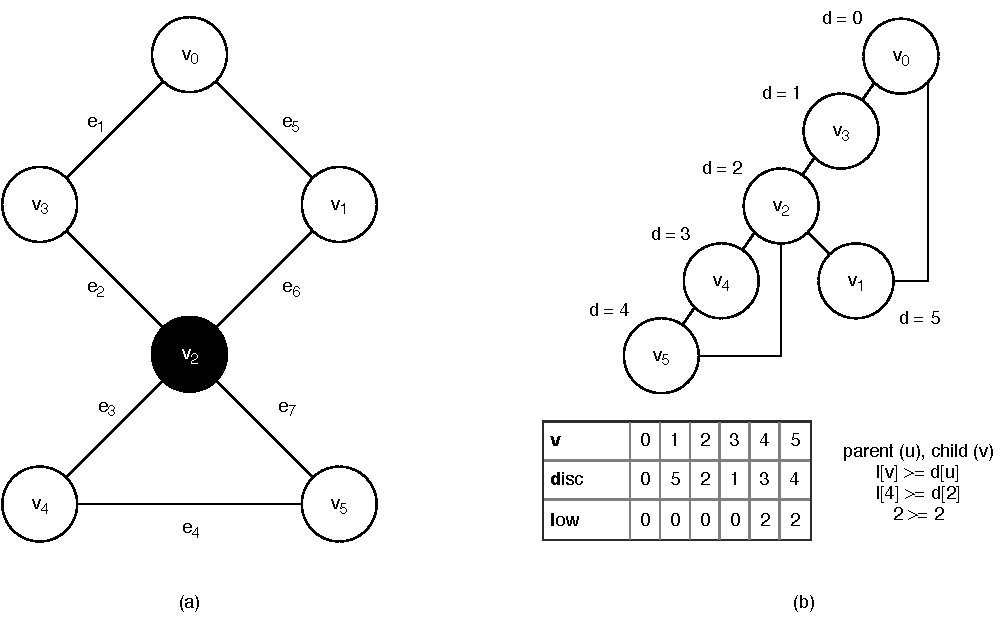
\includegraphics[width=0.8\linewidth]{document/ArticulationPoints/images/graph-dfs}
	\caption{Punto de articulación. (a) Grafo con punto de articulación en el vértice \( v_2 \). (b) Árbol DFS del grafo y \textit{Back Edge.}}
	\label{fig:graph-dfs}
\end{figure}

El siguiente código en JavaScript, es la implementación del algoritmo de Tarjan. No sé recomienda ejecutarlo en ambientes de producción, se desarrollo en este lenguaje por su facilidad de ejecutar.
\lstinputlisting[label=JSTarjan, caption=Código en JavaScript, language=JavaScript]{document/ArticulationPoints/code/Tarjan.js}
